%!TEX root=../../main.tex

\section{Exercises}
\label{exercisesChapterSimpleLogisticRegression}

%_______________
\subsection{Introduction to simple logistic regression}

% 1 ODD 
\eoce{\qt{Odds and probabilities} Suppose an experiment consists of rolling a fair six-sided die once. 
  \begin{parts}
  \item What are the odds of rolling a six?
  \item What are the odds of rolling an even number?
  \item  Explain to someone who  has not taken statistics the interpretation of the odds versus the probability of rolling an even number.
  \end{parts}
}{}

% 2 EVEN
\eoce{\qt{Diabetes} In the United States, approximately 9\% of the population have diabetes.
  \begin{parts}
  \item What are the odds that a randomly selected member of the US population has diabetes?
  \item Suppose that in a primary care clinic, the prevalence of diabetes among the patients seen in the clinic is 12\%.  What is the probability that a randomly selected patient in the clinic has diabetes?  What are the odds of diabetes for that patient?
  \item If in a particular population the probability of diabetes is twice what it is in the general population, does the odds of diabetes double?
  \end{parts}
}{}

% 3 Odd
\eoce{\qt{Hyperuricemia and BMI, I} The fourth quintile of BMI in 
Figure~\ref{figure:huBMIQuintiles} ranges from $25.02$ to $26.64$ meters per $\text{(kg)}^2$ and has median value $25.93$.  
    \begin{parts}
    \item Calculate the estimated conditional odds and probability of hyperuricemia for the value \texttt{bmi} = $25.93$ using the model shown in
Figure~\ref{figure:bmiHyperuricemiaLogRegCoeff}. 
      \item Does the conditional probability of hyperuricemia calculated for the fourth quintile in Figure~\ref{figure:huBMIQuintiles} lie above or below the value estimated in part (a)?
    \end{parts}
}{}

% 4 EVEN
\eoce{\qt{Interpreting model parameters, Part I} The curve with the solid line in Figure~\ref{figure:probVsPredictor} corresponds to $\beta_0 = -3.0$ and $\beta_1 = 0.6$.
\begin{parts}
\item Using the formula for the curve, calculate the odds ratio for $E$ comparing $x = 6$ to $x = 4$.
\item Using this curve, calculate the relative risk of the event $E$ comparing the value of the predictor $x = 6$ versus $x = 4$.
\item What role does the intercept play in the two calculations in (a) and (b)?

\end{parts}
}{}

\eoce{\qt{Interpreting model parameters, Part II} The curve with the dotted line in Figure~\ref{figure:probVsPredictor} corresponds to $\beta_0 = 3.0$ and $\beta_1 = -0.6$.
\begin{parts}
\item Using the formula for this curve, calculate the odds ratio for $E$ comparing $x = 6$ to $x = 4$.
\item Calculate the relative risk of the event $E$ comparing the value of the predictor $x = 6$ versus $x = 4$.

\item What role does the intercept play in the two calculations in (a) and (b)?
\end{parts}
}{}


\eoce{\qt{CPR and survival to discharge, Part I} Suppose a logistic regression  model is used to estimate the association of the odds of surviving to discharge and the number of minutes  cardiopulmonary resuscitation (CPR) was given to patients admitted to an emergency room following cardiac arrest.  The response variable is survival to hospital discharge and the predictor is length of CPR in minutes.  In the model the coefficient of CPR time is -0.065.

  \begin{parts}

  \item Is increased time of CPR associated with a increase or decrease in the chance of survival to discharge?

  \item What is OR for survival to discharge comparing someone given CPR for  10 versus someone requiring 20 minutes of CPR time?

  \item In three sentences, describe your answers to parts a and b  to someone who has not studied statistics.

  \end{parts}
}{}

\eoce{\qt{CPR and survival to discharge, Part II} Suppose in the model for CPR and survival to discharge the coefficient of the intercept is 1.44. 
  \begin{parts}
  \item What are the odds of survival to discharge for someone requiring 10 minutes of CPR?
  \item Check your answer to Part I(b) by calculating the odds of survival to discharge for someone requiring 20 minutes of CPR and using it and the answer to (a) above to calculate the the OR for 10 versus 20 minutes of CPR.
  \item Calculate the estimated probabilities of survival to discharge for 10 and 20 minutes of CPR.
  \item What is the relative risk of survival to discharge, comparing 10 versus 20 minutes of CPR.
  \item Explain the distinction between the estimated OR and RR to someone who has not taken statistics.
  \end{parts}
}{}

\eoce{\qt{Hyperuricemia and dietary magnesium, Part I} The investigators who studied hyperuricemia  in China also measured daily dietary intake of magnesium. The logistic regression model for the association between hyperuricemia (the response variable) and dietary magnesium (the predictor, measured in units of 1 gram) is given in the table below.
 % \begin{figure*}[ht]
%\centering
  \begin{center}
\begin{tabular}{rrr}
  \hline
  & Intercept & Magnesium (per gram)  \\ 
  \hline
 & -1.46 & 0.033  \\ 
   \hline
\end{tabular}
\end{center}
%\caption{Estimated logistic regression coefficients, 
      % the association of hyperuricemia with dietary magnesium} 
     %  \label{figure:magnesiumHyperuricemiaLogRegCoef}
%\end{figure*}
       
\begin{parts}
\item Write the algebraic form of the logistic regression model for the association of hyperuricemia and dietary magnesium.

\item Is dietary magnesium positively or negatively associated with hyperuricemia?

\item What are the predicted odds of hyperuricemia for someone with 0.5 grams magnesium/day in their diet?

\item By what factor will predicted odds change if a person with 0.5gm of dietary magnesium reduces their intake by 50\%? 

\item What is the predicted probability of hyperuricemia for someone with 0.5gm
magnesium in their daily diet.

\item By what factor will predicted probability change if a person with 0.5gm of dietary magnesium reduces their intake by 50\%? 

\end{parts}
}{}

\eoce{\qt{Hyperuricemia and age}The logistic regression model for the association between hyperuricemia (the response variable) and age (the predictor, measured years) is given in the table below.
 % \begin{figure}[ht]
%\centering
  \begin{center}
\begin{tabular}{rrr}
  \hline
  & Intercept & Age (per year)  \\ 
  \hline
 & -1.089 & -0.007  \\ 
   \hline
\end{tabular}
\end{center}
%\caption{Estimated logistic regression coefficients, 
 %      the association of hyperuricemia with dietary magnesium} 
     %  \label{figure:ageHyperuricemiaLogRegCoeff}
%\end{figure}

\begin{parts}
\item Write the algebraic form of the logistic regression model for the association of hyperuricemia and age.

\item Is increasing age associated with an increase or decrease in the odds of hyperuricemia?

\item What are the predicted odds of hyperuricemia for a 50 year old from this population.  

\item By what factor will predicted odds differ between someone who is 30 and someone who is 50 years old. 

\item What is the predicted probability of hyperuricemia for a 50 year old?

\item What is the relative risk of hyperuricemia, comparing a 50 year old to a 30 year old?

\end{parts}
}{}

% solutions checked to here, 21 feb 2023

\subsection{Inference for Simple Logistic Regression}


\eoce{\qt{Logistic Regression short answer, I} For the true/false questions, provide a reason for you answer.  The short answer questions can usually be answered in 2 - 3 sentences.

\begin{parts}

\item True or false: Equation~\ref{eqn:probLogisticRegression} can always be used to estimate probabilities after fitting a logistic regression.

\item True or false: Using the results of a logistic regression, the odds ratio for two cases with numerical predictor values 100 and 110 will be the same for two different cases with predictor values 20 and 30.

\item In your own words, explain the concepts of the odds of an event.

\item Suppose in a dataset, a binary outcome is a response variable and there is a single numerical predictor.  True or false: if both linear and logistic regression models are fit to the data, the estimated slopes will have the same interpretation.

\end{parts}

}{}  

\eoce{\qt{Logistic Regression short answer, II} For the true/false questions, provide a reason for you answer.  The short answer questions can usually be answered in 2 - 3 sentences.

\begin{parts}

\item True or false:  Since the sampling distributions of the estimated parameters in a logistic regression do not depend on sample size, logistic regression can be fit to arbitrarily small data sets.

\item Suppose a logistic regression has been fit to a dataset and the estimated slope parameter for the log(odds) is $0.750$.  Are increasing values of the predictor associate with increased or decreased risk of the outcome?

\item  Suppose the dataset was gathered in a prospective study with exposure based sampling.  Is the information in part~(b) sufficient to estimate the probability of the outcome, given a value of the exposure variable?

\item If the standard error of the estimate in part~(b) is $0.650$, does the study provide strong evidence for the association of the predictor with outcome? 

\end{parts}

}{}

\eoce{\qt{TB treatment interruption and secondary education} The two-way table in Figure~\ref{figure:tbInterruptionEduExample} summarizes the data
used to estimate the model in Figure~\ref{figure:tbInterruptionEduLogReg} in Example~\ref{example:tbInterruptionEducation}. \textbf{replace this problem; it duplicates later material}

\begin{parts}

\item Use the methods outlined in Section~\ref{inferenceOddsRatios} to calculate a  $95\%$ confidence interval for the OR in part~(a).

\item  Conduct a test of $H_0:\text{OR} = 1$ using the confidence interval in part~(a).

\item  Explain why the results of this problem are similar to those obtained in Example~\ref{example:tbInterruptionEducation}.

\end{parts}

}{}


\eoce{\qt{Hyperuricemia and dietary magnesium, II} The table below shows more detail about the logistic regression model for hyperuricemia and dietary magnesium.  

  % latex table generated in R 4.1.0 by xtable 1.8-4 package
% Tue Aug 31 13:45:18 2021
%\begin{table}[ht]
  % edited to reduce digits
%\centering
  \begin{center}
  \begin{tabular}{rrr}
  \hline
 & Estimate & Std. Error   \\ 
  \hline
(Intercept) & -1.462 & 0.229   \\ 
  magnesium.intake.gm & 0.033 & 0.526   \\ 
   \hline
\end{tabular}
\end{center}
%\end{table}

\begin{parts}

\item What is the value of the $z$-statistic used to test the null hypothesis of no association between hyperuricemia and dietary magnesium?

\item Do the data show a statistically significant association between hyperuricemia and  dietary magnesium?

\item Construct a 95\% confidence interval for the coefficient of dietary magnesium.  What is the interpretation of the interval?

\item Construct a 95\% confidence interval for the odds ratio comparing  individuals with 0.75gm versus 0.25gm of daily dietary magnesium.

\end{parts}
}{}

\eoce{\qt{Hyperuricemia and age, II}The table below shows additional details of the logistic regression model for the association between hyperuricemia and age.  

% latex table generated in R 4.1.0 by xtable 1.8-4 package
% Tue Aug 31 14:22:08 2021
  % edited to reduce significant digits
%\begin{table}[ht]
%\centering
  \begin{center}
  \begin{tabular}{rrr}
  \hline
 & Estimate & Std. Error  \\ 
  \hline
(Intercept) & -1.089 & 0.817 \\ 
  age & -0.007 & 0.015  \\ 
   \hline
\end{tabular}
\end{center}
%\end{table}

\begin{parts}

\item What is the value of the $z$-statistic for testing the null hypothesis of no association between hyperuricemia and age?

\item Do the data show a statistically significant relationship between hyperuricemia and age?

\item Construct and interpret a 95\% confidence interval for the coefficient of age.

\item Find a 95\% confidence interval for the odds ratio for hyperuricemia comparing a 75 versus a 50 year old individual.
\end{parts}
}{}

\eoce{\qt{Rare events \label{rare_event_sample_size}}
Public health research often involves the study of the association between an exposure and rare events. Radiation of certain wavelengths, called ionizing radiation, may have sufficient energy to damage DNA in a way that may lead to cancer.  Radon is a form of ionizing radiation that is found in many homes and is known to cause lung cancer.  It is produced from a natural breakdown of uranium in soil, rock and water.  Radon is  measured in in picocuries per liter, (pCI/L), and the US Environmental Protection Agency considers an average exposure of 4 pCI/L a safe level for adults.

Suppose a team is studying the possibility that pediatric leukemia may be associated with a low dose of radon exposure during pregnancy. In $10,000$ randomly selected homes in a metropolitan area, the team records radon levels (in picocuries per liter, pCI/L) and whether or not a woman in the home is pregnant. One year later the team records whether or not the recorded pregnancies led to a successful birth and, if so, the health status of the infant.  

\begin{parts}

\item Suppose $1,500$ of the women in the homes successfully delivered infants (all singleton births) and of those infants, $0.25\%$ of the infants were diagnosed with a from of leukemia.  Does the team have sufficient data to study the association of the dose of radon and the diagnosis of leukemia in an infant using logistic regression?

\item Assume that the estimated proportions of successful pregnancies and a subsequent diagnosis of leukemia in an infant are accurate in this metropolitan area.  What is the minimum number of homes the team should sample to reliably use logistic regression to study a dose-response relationship between infant leukemia and radon?

\item Suggest a way that the data from the original study be used to calculate a larger sample size that would be more likely to yield enough events to use logistic regression in this setting, and calculate that sample size using your suggestion.

\end{parts}
}{}

\eoce{\qt{Challenger disaster, Part I\label{challenger_disaster_model_select}} 
On January 28, 1986, a routine launch was anticipated for the Challenger space 
shuttle. Seventy-three seconds into the flight, disaster happened: the shuttle 
broke apart, killing all seven crew members on board. An investigation into the 
cause of the disaster focused on a critical seal called an O-ring, and it is 
believed that damage to these O-rings during a shuttle launch may be related to 
the ambient temperature during the launch. The table below summarizes 
observational data on O-rings for 23 shuttle missions, where the mission order 
is based on the temperature at the time of the launch. \emph{Temp} gives the 
temperature in Fahrenheit, \emph{Damaged} represents the number of damaged O-
rings, and \emph{Undamaged} represents the number of O-rings that were not 
damaged.
\begin{center}
\begin{tabular}{l rrrrr rrrrr rrrrr rrrrr rrr}
\hline
\vspace{-3.1mm} \\
Shuttle Mission   & 1  & 2 & 3 & 4 & 5 & 6 & 7 & 8 & 9 & 10 & 11 & 12 \\
\hline
\vspace{-3.1mm} \\
Temperature       & 53 & 57 & 58 & 63 & 66 & 67 & 67 & 67 & 68 & 69 & 70 & 70  \\
Damaged           & 5  & 1 & 1 & 1 & 0 & 0 & 0 & 0 & 0 & 0 & 1 & 0 \\
Undamaged         & 1  & 5 & 5 & 5 & 6 & 6 & 6 & 6 & 6 & 6 & 5 & 6 \\
\hline
\\ 
\cline{1-12}
\vspace{-3.1mm} \\
Shuttle Mission   & 13 & 14 & 15 & 16 & 17 & 18 & 19 & 20 & 21 & 22 & 23 \\
\cline{1-12}
\vspace{-3.1mm} \\
Temperature       & 70 & 70 & 72 & 73 & 75 & 75 & 76 & 76 & 78 & 79 & 81 \\
Damaged           & 1  & 0 & 0 & 0 & 0 & 1 & 0 & 0 & 0 & 0 & 0 \\
Undamaged         & 5  & 6 & 6 & 6 & 6 & 5 & 6 & 6 & 6 & 6 & 6 \\
\cline{1-12}
\end{tabular}
\end{center}
\begin{parts}
\item Each column of the table above represents a different shuttle mission. 
Examine these data and describe what you observe with respect to the 
relationship between temperatures and damaged O-rings.
\item Failures have been coded as 1 for a damaged O-ring and 0 for an undamaged 
O-ring, and a logistic regression model was fit to these data. A summary of this 
model is given below. Describe the key components of this summary table in words.
\begin{center}
\begin{tabular}{rrrrr}
  \hline
            & Estimate & Std. Error & z value   & Pr($>$$|$z$|$) \\ 
  \hline
(Intercept) & 11.6630  & 3.2963     & 3.54      & 0.0004 \\ 
Temperature & -0.2162  & 0.0532     & -4.07     & 0.0000 \\ 
  \hline
\end{tabular}
\end{center}
\item Write out the logistic model using the point estimates of the model 
parameters.
\item Based on the model, do you think concerns regarding O-rings are justified? 
Explain.
\end{parts}
}{}

\eoce{\qt{Hyperuricemia and BMI, II}

\begin{parts}

\item  Use the entries in Figure~\ref{figure:bmiHyperuricemiaLogReg} to calculate a 95\% confidence interval for the odds ratio for hyperuricemia comparing two individuals with BMI 27 and 23.

\item Ignoring issues of multiple testing, can the interval be used to support the claim that the data show that a BMI of 27 puts someone at significantly higher risk of hyperuricemia that someone with a BMI of 23? 

\end{parts}
}{}


\eoce{\qt{Challenger disaster, Part II\label{challenger_disaster_predict}} 
Exercise~\ref{challenger_disaster_model_select} introduced us to O-rings that 
were identified as a plausible explanation for the breakup of the Challenger 
space shuttle 73 seconds into takeoff in 1986. The investigation found that the 
ambient temperature at the time of the shuttle launch was closely related to the 
damage of O-rings, which are a critical component of the shuttle. See this 
earlier exercise if you would like to browse the original data.
\begin{center}
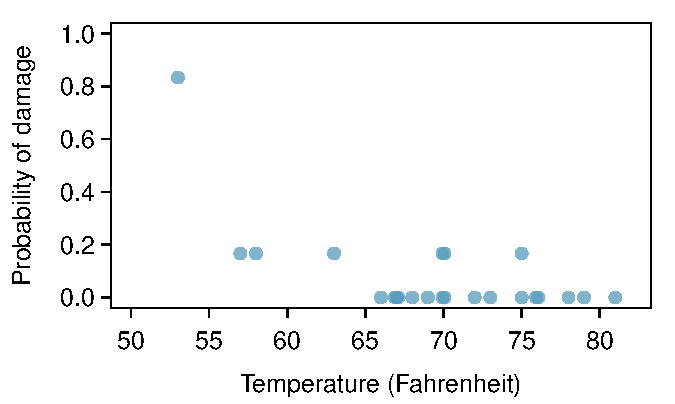
\includegraphics[width=0.6\textwidth]{ch_logistic_regression_oi_biostat/figures/eoce/challenger_disaster_predict/challenger_disaster_damage_temp.pdf} 
\end{center}
\begin{parts}
\item The data provided in the previous exercise are shown in the plot. The logistic 
model fit to these data may be written as
\begin{align*}
\log\left( \frac{\hat{p}}{1 - \hat{p}} \right) = 11.6630 - 0.2162\times Temperature
\end{align*}
where $\hat{p}$ is the model-estimated probability that an O-ring will become 
damaged. Use the model to calculate the probability that an O-ring will become 
damaged at each of the following ambient temperatures: 51, 53, and 55 degrees 
Fahrenheit. The model-estimated probabilities for several additional ambient 
temperatures are provided below, where subscripts indicate the temperature:
\begin{align*}
&\hat{p}_{57} = 0.341
  && \hat{p}_{59} = 0.251
  && \hat{p}_{61} = 0.179
  && \hat{p}_{63} = 0.124 \\
&\hat{p}_{65} = 0.084
  && \hat{p}_{67} = 0.056
  && \hat{p}_{69} = 0.037
  && \hat{p}_{71} = 0.024
\end{align*}
\item Add the model-estimated probabilities from part~(a) on the plot, then 
connect these dots using a smooth curve to represent the model-estimated 
probabilities.
\item Describe any concerns you may have regarding applying logistic regression 
in this application, and note any assumptions that are required to accept the 
model's validity.
\end{parts}

}{}


\subsection{Multiple logistic regression}


%\begin{comment}


\eoce{\qt{Risk of fracture\label{exercise:fractureRiskGlow}}

Osteoporosis a bone disease characterized by decreasing bone mineral density and bone mass and is associated with a higher risk of fractures (broken bones) after falls.  The Global Longitudinal Study of Osteoporosis in Women (GLOW) collected data on over 60,000 women over 55 years of age diagnosed with osteoporosis. This exercise uses data from the study provided in Hosmer, Lemeshow and Sturdivant\footfullcite{hosmer2013applied}, which contains additional information about the study. Briefly, the study followed the participants during the study period, recording potential predictors of fracture at enrollment and the first occurrence of a fracture during the follow-up period.  The GLOW data can be found in the \textsf{R} package APLORE.

The data in this exercise contains information from 500 participants and includes the occurrence of a fracture and selected possible risk factors.  This sample was drawn by Hosmer, Lemeshow and Sturdivant from the full dataset by oversampling participants with fractures and undersampling those without fractures, since only approximately 4\% of the participants experienced fractures.

Figure~\ref{glowFracAge} shows a logistic regression model with response variable whether or not the participant experienced a fracture during the study and predictors the factor variable the presence of a prior fracture (coded Yes, No) and age of the participant, in years.


% Tue Oct 17 13:58:34 2023
\begin{figure}[ht]
\centering
\begin{tabular}{rrrrr}
  \hline
 & Estimate & Std. Error & z value & Pr($>$$|$z$|$) \\ 
  \hline
(Intercept) & -4.214 & 0.848 & -4.97 & 0.000 \\ 
  priorfracYes & 0.839 & 0.234 & 3.58 & 0.000 \\ 
  age & 0.041 & 0.012 & 3.38 & 0.001 \\ 
   \hline
\end{tabular}
\caption{Logistic Regression for fracture with predictors age 
       and presence of prior fracture} 
\label{glowFracAge}
\end{figure}

\begin{parts}

\item For a 60 year old women use the model to estimate the odds ratio for the occurrence  of a fracture comparing women with a prior fracture to those without a prior fracture.

\item For a woman who has not had a prior fracture, estimate the odds ratio for the occurrence of a fracture, comparing a 75 year old woman with one who is 65.

\item Does the design of the study and this sample of 500 participants support the estimates of ORs in parts~(a) and (b)?  Justify your answer.

\item Can the data from the study be used to estimate prevalence differences and ratios in parts~(a) and (b)? Justify your answer.

\end{parts}

}{}

%\end{comment}

\eoce{\qt{HIV test status and TB treatment interruption. \label{exerise:tbInterruption}}

Show that the conditions for a $\chi^2$ test are met for the data displayed in Figure~\ref{figure:tbInterruptionEduExample}.

}{}

\eoce{\qt{Female horseshoe crabs, color and satellites. \label{exercise:colorsSatellitesCrabsChiSq}}

Show that the conditions for a $\chi^2$ test are met for the data displayed in Figure~\ref{figure:colorSatelliteCrabs}.

}{}

\eoce{\qt{Emergency room outcomes in Denmark, I
   \label{exercise:mort1000Triage}}

An important problem in emergency medicine is the prioritization of high-risk patients. Traditional triage algorithms classify patients into categories based on vital signs (such as heart rate and level of consciousness) in addition to the patient's reason for seeking medical care: "red" (life-threatening), "orange" (seriously ill), "yellow" (ill), "green" (needs assessment), and "blue" (minor complaints). A study in Denmark\footfullcite{kristensen2017routine} studied the association of triage score and other variables with 30 day mortality in a dataset of 12,661 individuals\footfullcite{Data available at DOI:10.5061/dryad.m2bq5} treated in the Emergency Department (ED) of  Nordsj{\ae}lland University Hospital in Denmark.  

The model in Figure~\ref{figure:mort30TriageSample1000} is the result of fitting a logistic regression with response variable 30-day mortality (0 = alive 30 days a after admission) and predictor triage score in a random sample of 1,000 cases from the 5,371 participants in the primary dataset used for initial model building.  In this sample of 1,000, there were 62 deaths within 30 days from admission to the ED.

Individuals classified as category blue were not included in the study.

% latex table generated in R 4.1.2 by xtable 1.8-4 package
% Mon Jun 27 09:05:25 2022
\begin{figure}[ht]
\centering
\begin{tabular}{rrrrr}
  \hline
 & Estimate & Std. Error & z value & Pr($>$$|$z$|$) \\ 
  \hline
(Intercept) & -1.551 & 0.416 & -3.73 & 0.000 \\ 
  triageorange & -0.958 & 0.474 & -2.02 & 0.043 \\ 
  triageyellow & -1.290 & 0.468 & -2.76 & 0.006 \\ 
  triagegreen & -1.585 & 0.518 & -3.06 & 0.002 \\ 
   \hline
\end{tabular}
\caption{Logistic regression with response 30 day mortality and
       predictor triage level, using a random sample of 1,000 cases 
       from Danish ED study primary cohort.} 
\label{figure:mort30TriageSample1000}
\end{figure}

\begin{parts}

\item What is the reference category in the regression?

\item Is the pattern in the estimates of the coefficients consistent with traditional triage coding?

\item Write the equation for the model.

\item Does the intercept have an interpretation in this model?  If so, what is its interpretation?

\item What is the estimated OR and 95\% confidence interval for 30 day mortality, comparing category "yellow" with "red"?

\item What is the OR for 30 day mortality, comparing category "yellow" with "orange"?

\end{parts}

}{}

\eoce{\qt{Emergency room outcomes in Denmark, II
\label{exercise:mortTriageColorTable}}

Figure\ref{figure:tableTriageMort30Sample1000} is a contingency table showing the association between 30 day mortality and triage classification for the data used in Exercise\ref{exercise:mort1000Triage}.

% latex table generated in R 4.1.2 by xtable 1.8-4 package
% Mon Jun 27 09:41:20 2022
\begin{figure}[ht]
\centering
\begin{tabular}{rrrr}
  \hline
 & 0 & 1 & Sum \\ 
  \hline
red & 33 & 7 & 40 \\ 
  orange & 258 & 21 & 279 \\ 
  yellow & 394 & 23 & 417 \\ 
  green & 253 & 11 & 264 \\ 
  Sum & 938 & 62 & 1000 \\ 
   \hline
\end{tabular}
\caption{Contingency table of 30 day mortality by triage classification,
       Danish ED study, random sample of 1,000 participants} 
\label{figure:tableTriageMort30Sample1000}
\end{figure}

\begin{parts}

\item Show that the table can be used to calculate the estimate of  the intercept given in Figure~\ref{figure:mort30TriageSample1000}.

\item The data in the table can be used to estimate each of the coefficients in the logistic model. Show that it can be used to calculate the estimate of the coefficient for the triage category "green".

\item Can the estimates of the standard errors in Figure~\ref{figure:mort30TriageSample1000} be calculated directly from the table?

\end{parts}
}{}

\eoce{\qt{Emergency room outcomes in Denmark, III
   \label{exercise:mortTriageAgeSex1000}}

The dataset used in Exercise~\ref{exercise:mort1000Triage} also contains the age and sex of the participants.  Figure~\ref{figure:mort30TriageAgeSexSample1000} shows the logistic model in which age in years and sex have been added to the traditional triage coding.

% latex table generated in R 4.1.2 by xtable 1.8-4 package
% Mon Jun 27 09:12:22 2022
\begin{figure}[ht]
\centering
\begin{tabular}{rrrrr}
  \hline
 & Estimate & Std. Error & z value & Pr($>$$|$z$|$) \\ 
  \hline
(Intercept) & -5.560 & 0.880 & -6.32 & 0.000 \\ 
  triageorange & -1.062 & 0.501 & -2.12 & 0.034 \\ 
  triageyellow & -1.245 & 0.494 & -2.52 & 0.012 \\ 
  triagegreen & -1.489 & 0.543 & -2.74 & 0.006 \\ 
  age & 0.058 & 0.010 & 5.89 & 0.000 \\ 
  sexmale & 0.009 & 0.277 & 0.03 & 0.974 \\ 
   \hline
\end{tabular}
\caption{Logistic regression with response 30 day mortality and
       predictors triage level, age and sex, using a random sample of 1,000 cases 
       from Danish ED study.} 
\label{figure:mort30TriageAgeSexSample1000}
\end{figure}

\begin{parts}

\item Does the intercept in this model have an interpretation?  If so, what is the interpretation?

\item Is increasing age associated with in increase or decrease in the risk of 30 day mortality?

\item The residual deviance for the model in Figures~\ref{figure:mort30TriageAgeSexSample1000} and \ref{figure:mortTriage1000} are, respectively, $407.58$ and $463.60$.  Conduct a test of the null hypothesis that the pair of variables \var{age} and \var{sex} do not add useful information to a model based on triage score alone.  

\item Based on the estimated model and your answers to the above, do you believe that both age and sex should be retained in the model?  Explain your answer.

\end{parts}

}{}

\eoce{\qt{Interaction in logistic regression, I
   \label{exercise:BMISexInteractionModel}}

The interaction term in the model given in Equation~\ref{eqn:huBmiSexInteractionLogReg} would not be retained in a model with BMI and sex, but it is instructive to explore the implications of an interaction when estimating ORs.

\begin{parts}

\item Calculate the estimated OR for hyperuricemia for two males with BMI 33.2 vs 30. 

\item Repeat the calculation for two females.

\item How do these estimates differ from the corresponding ORs when using the model without an interaction in Figure~\ref{figure:huBmiSexLogReg}?

\end{parts}

}{}    

\eoce{\qt{Interaction in logistic regression, II
   \label{exercise:BMISexInteractionDirect}}

Adding a term to a logistic regression is the preferred method for examining interactions.  In some settings it is possible to compare the separate estimates of log odds ratios from subsets without imposing a model. 

\begin{parts}

\item Use the information in Figures~\ref{figure:bmiHyperuricemiaFemalesLogReg} and \ref{figure:bmiHyperuricemiaMalesLogReg} to calculate the two variances of the log odds estimates of hyperuricemia for females and males. 

\item Calculate the variance and standard deviation of the difference between the two estimates of log odds.

\item Conduct a test of the null hypothesis that the difference between the two estimates is 0.

\item Discuss the advantages and disadvantages of this approach compare to using the model in Figure~\ref{eqn:huBmiSexInteractionLogReg} 

\end{parts}

}{}

\begin{comment}

*** removing this and the next exercise for now.  Not very good, not sure whether they ***  can be improved.


\eoce{\qt{Smoking and marijuana use, I
   \label{exercise:smokingMarij}}

Figure~\ref{figure:smoke100RegMarijuana} shows the association between smoking at least 100 cigarettes a year and regular marijuana use in a sample of 500 participants from the NHANES data in the package \texttt{oibiostat}.  Figure~\ref{figure:marijSmokelogreg} below shows a logistic model fit to the same data, with response regular marijuana use and the smoking variable (\texttt{Smoke100}) as the predictor.

% latex table generated in R 4.1.2 by xtable 1.8-4 package
% Wed Jun 29 14:28:14 2022
\begin{figure}[ht]
\centering
\begin{tabular}{rrrrr}
  \hline
 & Estimate & Std. Error & z value & Pr($>$$|$z$|$) \\ 
  \hline
(Intercept) & -1.882 & 0.224 & -8.41 & 0.000 \\ 
  Smoke100Yes & 1.568 & 0.284 & 5.53 & 0.000 \\ 
   \hline
\end{tabular}
\caption{Logistic regression with response regular marijuana use
       and predictor Smoke100} 
\label{figure:marijSmokelogreg}
\end{figure}

Figure~\ref{figure:marijSmokeAgeGenderWorklogreg} expands the logistic regression model by adding Age, Gender (biological sex, coded "male", "female") and the categorical variable Work (coded "Looking", "Not Working", "Working").

% latex table generated in R 4.1.2 by xtable 1.8-4 package
% Wed Jun 29 15:00:01 2022
\begin{figure}[ht]
\centering
\begin{tabular}{rrrrr}
  \hline
 & Estimate & Std. Error & z value & Pr($>$$|$z$|$) \\ 
  \hline
(Intercept) & -3.472 & 1.226 & -2.83 & 0.005 \\ 
  Smoke100Yes & 1.604 & 0.292 & 5.49 & 0.000 \\ 
  Age & -0.013 & 0.013 & -0.99 & 0.320 \\ 
  Gendermale & 0.893 & 0.291 & 3.07 & 0.002 \\ 
  WorkNotWorking & 2.173 & 1.134 & 1.92 & 0.055 \\ 
  WorkWorking & 1.480 & 1.107 & 1.34 & 0.181 \\ 
   \hline
\end{tabular}
\caption{Logistic regression with response regular marijuana use
       and predictors Smoke100, Age, Gender (biological sex) and work status} 
\label{figure:marijSmokeAgeGenderWorklogreg}
\end{figure} 

\begin{parts}

\item  Show that the OR for regular marijuana use comparing smokers to non-smokers from the logistic regression in Figure~\ref{figure:marijSmokelogreg} is the same as the one that can be calculated from the two-way table.

\item Show that a 95\% confidence interval for the log(OR) comparing smokers to non-smokers calculated from the logistic regression in Figure~\ref{figure:marijSmokelogreg} is approximately equal to the interval calculated from the contingency table using the formula in Section~\ref{section:inferenceOddsRatios}.

\item Write a brief description of what can be learned from the two regression models for someone who has not studied statistics.


\end{parts}

}{}
\eoce{\qt{Smoking and marijuana use, II
   \label{exercise:smokingMarijSrvYr}}

When survey data are collected in different time  periods,  it is  important to know if any estimated associations might differ according to the data collection period.  The NHANES data was collected in two surveys, one in 2009 - 2010 and a second in 2011 - 2012.  The dataset used to fit the model in Exercise~\ref{exercise:smokingMarij} includes a categorical variable \var{SurveyYr} with two levels denoting year of the participant's data.  

Write down a logistic regression model that can be used to check whether the association between regular marijuana use and smoking differed the survey period.

}{}

\end{comment}

\begin{comment}

Additional potential exercises with these data

- Something similar to Challenger data question

GoF fails because of some zero cateories

\end{comment}

